% Simplified Beginner-Friendly GNU Radio Workshop Slides
\documentclass[aspectratio=169,12pt]{beamer}

% Theme
\usetheme{Madrid}
\usecolortheme{whale}

% Packages
\usepackage{graphicx}
\usepackage{tikz}
\usepackage{listings}
\usepackage{amsmath,amssymb}
\usepackage{verbatim}
\usepackage{animate}
\usepackage{multicol}

% TikZ libraries
\usetikzlibrary{shapes,arrows,positioning,calc,shadows,patterns}
\usetikzlibrary{decorations.pathreplacing,decorations.pathmorphing}

% Custom colors
\definecolor{radioblue}{RGB}{0,123,255}
\definecolor{radiogreen}{RGB}{40,167,69}
\definecolor{radioorange}{RGB}{255,127,36}
\definecolor{radiopurple}{RGB}{128,0,128}
\definecolor{radiored}{RGB}{220,53,69}
\definecolor{radioyellow}{RGB}{255,193,7}
\definecolor{radiogray}{RGB}{108,117,125}

% Custom commands for visual elements
\newcommand{\highlight}[1]{\colorbox{yellow!30}{#1}}
\newcommand{\important}[1]{\textcolor{radioblue}{\textbf{#1}}}

% Title Information
\title{Welcome to the World of Software Defined Radio}
\subtitle{A Beginner's Journey with GNU Radio}
\author[Instructor]{Your Workshop Instructor}
\institute[GRCon]{GNU Radio Conference 2025}
\date{\today}

\begin{document}

% Title slide
\begin{frame}
\titlepage
\end{frame}

% Table of Contents
\begin{frame}{What We'll Cover Today}
\tableofcontents
\end{frame}

% Section 1: What is Radio?
\section{Understanding Radio Waves}

\begin{frame}{What Are Radio Waves?}
\begin{center}
\Large\textbf{Radio = Invisible Waves Through the Air}
\end{center}
\vspace{1em}

\begin{columns}
\column{0.5\textwidth}
\textbf{Like Sound Waves:}
\begin{itemize}
    \item Travel through space
    \item Have frequency (pitch)
    \item Have amplitude (volume)
\end{itemize}

\column{0.5\textwidth}
\textbf{But Different:}
\begin{itemize}
    \item Much faster
    \item Can carry data
    \item Need special equipment
\end{itemize}
\end{columns}
\end{frame}

\begin{frame}{Radio is Everywhere!}
\begin{center}
\Large\textbf{You Use Radio Every Day}
\end{center}
\vspace{1em}

\begin{itemize}
    \item WiFi (2.4 GHz, 5 GHz)
    \item Cell Phones (700 MHz - 2.6 GHz)
    \item Bluetooth (2.4 GHz)
    \item Car Keys (315/433 MHz)
    \item GPS (1.2/1.5 GHz)
    \item FM Radio (88-108 MHz)
\end{itemize}

\vspace{1em}
\begin{center}
\colorbox{yellow!20}{\parbox{0.8\textwidth}{\centering
\textbf{Fun Fact:} Your microwave oven uses the same frequency as WiFi!}}
\end{center}
\end{frame}

% Section 2: What is SDR?
\section{Software Defined Radio}

\begin{frame}{Traditional Radio vs SDR}
\begin{columns}
\column{0.5\textwidth}
\begin{center}
\textbf{\Large Traditional Radio}\\
\textcolor{radiogray}{Hardware Does Everything}
\end{center}
\begin{itemize}
    \item Fixed function
    \item Need new hardware for changes
    \item Limited flexibility
    \item Like a calculator
\end{itemize}

\column{0.5\textwidth}
\begin{center}
\textbf{\Large Software Defined Radio}\\
\textcolor{radioblue}{Software Does the Magic}
\end{center}
\begin{itemize}
    \item Flexible function
    \item Change with software
    \item Unlimited possibilities
    \item Like a computer
\end{itemize}
\end{columns}
\end{frame}

\begin{frame}{Why SDR is Amazing}
\begin{center}
\Large\textbf{One Device, Many Functions}
\end{center}
\vspace{1em}

With the same SDR hardware, you can:
\begin{itemize}
    \item Listen to FM radio
    \item Decode aircraft signals
    \item Receive weather satellites
    \item Build a walkie-talkie
    \item Track ships at sea
    \item Analyze WiFi
    \item And much more!
\end{itemize}

\vspace{1em}
\begin{center}
\colorbox{radiogreen!20}{\parbox{0.8\textwidth}{\centering
\textbf{It's like having a Swiss Army knife for radio!}}}
\end{center}
\end{frame}

% Section 3: GNU Radio Introduction
\section{Meet GNU Radio}

\begin{frame}{What is GNU Radio?}
\begin{center}
\Large\textbf{Your Free SDR Toolkit}
\end{center}
\vspace{1em}

\begin{columns}
\column{0.5\textwidth}
\textbf{GNU Radio is:}
\begin{itemize}
    \item Free and open source
    \item Visual programming tool
    \item Professional grade
    \item Community supported
\end{itemize}

\column{0.5\textwidth}
\textbf{You can:}
\begin{itemize}
    \item Build by connecting blocks
    \item See signals in real-time
    \item Process any radio signal
    \item Create your own blocks
\end{itemize}
\end{columns}

\vspace{1em}
\begin{center}
\colorbox{radioblue!20}{\parbox{0.8\textwidth}{\centering
\textbf{Think of it as LEGO blocks for radio systems!}}}
\end{center}
\end{frame}

\begin{frame}{GNU Radio Companion (GRC)}
\begin{center}
\Large\textbf{Visual Programming Interface}
\end{center}
\vspace{1em}

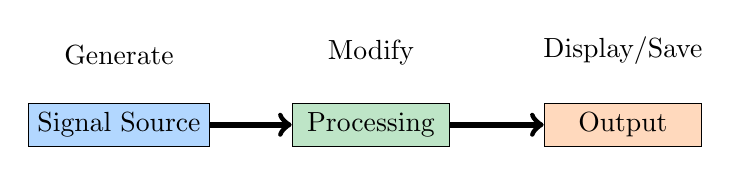
\begin{tikzpicture}[scale=0.8]
    % Blocks
    \node[draw, fill=radioblue!30, minimum width=2cm] (source) at (0,0) {Signal Source};
    \node[draw, fill=radiogreen!30, minimum width=2cm] (process) at (4,0) {Processing};
    \node[draw, fill=radioorange!30, minimum width=2cm] (sink) at (8,0) {Output};
    
    % Connections
    \draw[->, line width=2pt] (source) -- (process);
    \draw[->, line width=2pt] (process) -- (sink);
    
    % Labels
    \node[above] at (0,0.8) {Generate};
    \node[above] at (4,0.8) {Modify};
    \node[above] at (8,0.8) {Display/Save};
\end{tikzpicture}

\vspace{1em}
Key Concepts:
\begin{itemize}
    \item \textbf{Blocks:} Do specific tasks
    \item \textbf{Connections:} Pass data between blocks
    \item \textbf{Flow:} Data moves left to right
\end{itemize}
\end{frame}

% Section 4: Basic Concepts
\section{Core Concepts}

\begin{frame}{Understanding Frequency}
\begin{center}
\Large\textbf{Frequency = How Fast Waves Wiggle}
\end{center}
\vspace{1em}

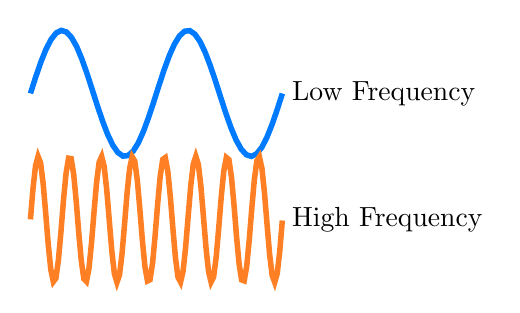
\begin{tikzpicture}[scale=0.8]
    % Low frequency
    \draw[radioblue, line width=2pt] plot[domain=0:4, samples=50] (\x, {sin(\x*180)});
    \node[right] at (4,0) {Low Frequency};
    
    % High frequency
    \draw[radioorange, line width=2pt] plot[domain=0:4, samples=100] (\x, {-2+sin(\x*720)});
    \node[right] at (4,-2) {High Frequency};
\end{tikzpicture}

\vspace{1em}
\begin{itemize}
    \item Measured in Hertz (Hz)
    \item 1 Hz = 1 wave per second
    \item MHz = Million waves per second
    \item GHz = Billion waves per second
\end{itemize}
\end{frame}

\begin{frame}{Sample Rate}
\begin{center}
\Large\textbf{How Often We Take Measurements}
\end{center}
\vspace{1em}

Think of it like video frame rate:
\begin{itemize}
    \item More frames = smoother video
    \item More samples = better signal quality
    \item Must sample at least 2x the highest frequency
    \item Common rates: 2.4 MHz, 10 MHz, 20 MHz
\end{itemize}

\vspace{1em}
\begin{center}
\colorbox{yellow!20}{\parbox{0.8\textwidth}{\centering
\textbf{Rule:} If you want to see a 1 MHz signal, sample at least at 2 MHz}}
\end{center}
\end{frame}

% Section 5: Hands-On
\section{Let's Build Something!}

\begin{frame}{Your First Flowgraph}
\begin{center}
\Large\textbf{Creating a Simple Tone Generator}
\end{center}
\vspace{1em}

Steps:
\begin{enumerate}
    \item Open GNU Radio Companion
    \item Add a Signal Source block
    \item Add an Audio Sink block
    \item Connect them together
    \item Set frequency to 440 Hz (musical note A)
    \item Click Run
    \item You'll hear a beep!
\end{enumerate}

\vspace{1em}
\begin{center}
\colorbox{radiogreen!20}{\parbox{0.8\textwidth}{\centering
\textbf{Congratulations! You just built your first radio system!}}}
\end{center}
\end{frame}

\begin{frame}{Common Blocks You'll Use}
\begin{center}
\Large\textbf{Your SDR Toolbox}
\end{center}
\vspace{0.5em}

\begin{columns}
\column{0.5\textwidth}
\textbf{Sources (Input):}
\begin{itemize}
    \item Signal Source
    \item File Source
    \item Audio Source
    \item RTL-SDR Source
\end{itemize}

\textbf{Sinks (Output):}
\begin{itemize}
    \item QT GUI Time Sink
    \item QT GUI Frequency Sink
    \item Audio Sink
    \item File Sink
\end{itemize}

\column{0.5\textwidth}
\textbf{Processing:}
\begin{itemize}
    \item Low Pass Filter
    \item Multiply
    \item Add
    \item FM Demod
\end{itemize}

\textbf{Control:}
\begin{itemize}
    \item Throttle
    \item Variable
    \item QT GUI Range
\end{itemize}
\end{columns}
\end{frame}

% Section 6: Next Steps
\section{Your Journey Forward}

\begin{frame}{What You Can Build}
\begin{center}
\Large\textbf{Project Ideas}
\end{center}
\vspace{1em}

\begin{columns}
\column{0.5\textwidth}
\textbf{Beginner Projects:}
\begin{itemize}
    \item FM radio receiver
    \item Audio spectrum analyzer
    \item Morse code generator
    \item Simple AM transmitter
\end{itemize}

\column{0.5\textwidth}
\textbf{Advanced Projects:}
\begin{itemize}
    \item Weather satellite decoder
    \item Aircraft tracker (ADS-B)
    \item Digital TV receiver
    \item Custom protocols
\end{itemize}
\end{columns}

\vspace{1em}
\begin{center}
\colorbox{radioblue!20}{\parbox{0.8\textwidth}{\centering
\textbf{Start simple, build confidence, then tackle bigger challenges!}}}
\end{center}
\end{frame}

\begin{frame}{Resources}
\begin{center}
\Large\textbf{Continue Learning}
\end{center}
\vspace{1em}

\textbf{Documentation:}
\begin{itemize}
    \item wiki.gnuradio.org - Official wiki
    \item tutorials.gnuradio.org - Step-by-step guides
\end{itemize}

\textbf{Community:}
\begin{itemize}
    \item discuss.gnuradio.org - Forum
    \item chat.gnuradio.org - Live chat
    \item GitHub - Code and examples
\end{itemize}

\textbf{Hardware:}
\begin{itemize}
    \item RTL-SDR (\$30) - Great starter
    \item HackRF (\$300) - Can transmit
    \item USRP (\$700+) - Professional
\end{itemize}
\end{frame}

\begin{frame}{Thank You!}
\begin{center}
\Huge\textbf{Questions?}
\vspace{2em}

\Large
Welcome to the GNU Radio Community!

\vspace{1em}
\normalsize
Remember: Every expert was once a beginner.\\
Don't be afraid to experiment and ask questions!

\vspace{2em}
\textbf{Happy SDR Exploring!}
\end{center}
\end{frame}

\end{document}